
% Definieren der Dokumentklasse
\documentclass[ngerman, 11pt]{article}

% T1 Font Encoding: Sonderzeichen ä,ü,ö,... als eigene Symbole
\usepackage[T1]{fontenc}

% UTF-8 Kodierung
\usepackage[utf8]{inputenc}

% Sprache Zeichensatz Deutsch
\usepackage[ngerman]{babel}

% Nutzen Mathematischer Symbole
\usepackage{amsmath}

% Nutzen weiterer Sonderzeichen
\usepackage{amssymb}

% Nutzen von Euro Symbolen
\usepackage{eurosym}

% Schriftart: helvet als Arial-Klon
\usepackage{helvet}
\renewcommand{\familydefault}{\sfdefault}

% Anpassen des Zeilenabstandes
\usepackage[singlespacing]{setspace}
\setstretch{1.454545454545455}% Faktor: 16pt/11pt = 1.454545454545455

% Rückung neuer Absätze
\setlength\parindent{0pt}

% Einbinden von Grafiken
\usepackage{graphicx}
\graphicspath{{../Karten}{.}{../Abbildungen}}

% Positionieren von Grafiken
\usepackage[export]{adjustbox}

% Definieren von Farben
\usepackage[table]{xcolor}% table Option für die Farbgestaltung von Tabellen
\definecolor{imreg}{RGB}{39, 89, 165}
\definecolor{urlcol}{RGB}{0, 0, 238}
\definecolor{imregdunkelrot}{RGB}{192, 0, 0}

% Erstellen von Verlinkungen und Pfaddarstellungen
\usepackage[obeyspaces]{url}
\usepackage{hyperref}
\hypersetup{
	breaklinks,
	colorlinks,
	linkcolor=black,
	urlcolor=urlcol
}

% Zuschneiden der Seite
\usepackage[paper=a4paper, top=40mm, bottom=27mm, left=20mm, right=20mm, headheight=61pt]{geometry}


\usepackage{pdflscape}

% Abstand der Bildüberschrift zum Bild
\setlength{\belowcaptionskip}{15pt}

% Nutzen und formattieren der Subfigure Umgebung
\usepackage{subcaption}
\captionsetup[subfigure]{labelformat=empty}


% Definieren von Kopf- und Fußzeile
\usepackage{fancyhdr}
\pagestyle{fancy}
\renewcommand{\headrulewidth}{1.5pt}
\let\oldheadrule\headrule\renewcommand{\headrule}{\color{imreg}\oldheadrule}
\renewcommand{\footrulewidth}{1.5pt}
\let\oldfootrule\footrule\renewcommand{\footrule}{\color{imreg}\oldfootrule}
\fancyhead[L]{\nouppercase \leftmark}
\fancyhead[C]{}
\fancyhead[R]{
\includegraphics[height=20mm]{imreg}}
\fancyfoot[L]{\color{black} Stand: \today}
\fancyfoot[C]{}
\fancyfoot[R]{\color{black} \thepage}



% Formatierung von Überschriften
\usepackage{titlesec}
% Hauptüberschriften
\titleformat{\section}
[block]% shape
{\color{imreg} \Large}% format
{\textbf{\thesection.}}% label
{11pt}% horizontal separation
{\textbf}% before-code
[]% after-code
% Hauptüberschriften
\titleformat{\subsection}
[block]% shape
{\color{imreg} \large}% format
{\textbf{\thesubsection.}}% label
{11pt}% horizontal separation
{\textbf}% before-code
[]% after-code
% Abstandsregel Hauptüberschriften
\titlespacing{\section}
{0pt}% left
{0pt}% before
{0pt}% after
\titlespacing{\subsection}
{0pt}% left
{0pt}% before
{0pt}% after


% Bild-, Tabellen- & Kartenüberschriften
\usepackage{caption}
\DeclareCaptionFormat{imregCaption}{\normalsize \color{imreg} \textbf{#1#2#3}}
\captionsetup{format=imregCaption, justification=centering, singlelinecheck=false}
%\setlength{\abovecaptionskip}{0pt}
%\setlength{\belowcaptionskip}{0pt}


% Formatieren der Listendarstellung
\usepackage{tocloft}
\renewcommand{\cftdot}{\ensuremath{}}
\renewcommand\cfttoctitlefont{\Large \bfseries \color{imreg}}
\renewcommand{\cftloftitlefont}{\Large \bfseries \color{imreg}}
\renewcommand{\cftlottitlefont}{\Large \bfseries \color{imreg}}

% Abbildungsverzeichnis
\renewcommand{\cftfigpresnum}{Abbildung }% Präfix
\settowidth{\cftfignumwidth}{Abbildung xx\quad}% Abstand bis Name
\setlength\cftfigindent{0pt}% Rückung

% Tabellenverzeichnis
\renewcommand{\cfttabpresnum}{Tabelle }
\settowidth{\cfttabnumwidth}{Tabelle xx\quad}
\setlength\cfttabindent{0pt}


% Zählfunktion für Karten
\newcommand{\listmapname}{Kartenverzeichnis}
\newlistof
{maps}% Zählvariable
{caption}% Platzhalter
{\Large \color{imreg} \listmapname}% Name
% Zählfunktion für Karten
\newcommand{\maps}[1]{%
	\refstepcounter{maps}
	\par\noindent \textbf{\large \color{imreg} Karte \themaps: #1}
	\addcontentsline{caption}{maps}{\normalsize Karte \themaps\quad\protect#1}\par}


% Befehl zum Erstellen einer Leerseite
\newcommand*\emptypage{\newpage\null\thispagestyle{empty}\newpage}

% Befehl zum Einbinden einer Karte
\newcommand{\karte}[3]{
	\vspace{15pt}
	\makebox[\linewidth][c]{
		\begin{subfigure}{0.61\textwidth}
			\centering
			\caption{\\#2}
			\includegraphics*[width=\textwidth, height=172mm, center]{#1} 
		\end{subfigure}
		\begin{subfigure}{0.61\textwidth}
			\centering
			\caption{\\#3}
			\includegraphics*[width=\textwidth, height=172mm, center]{#1_Delta}
		\end{subfigure}
	}
}



% Informationen für das Deckblatt
\title{M+E Osteuropaatlas}
\author{Simon Gräfe}


\usepackage{lipsum}

\usepackage{datetime}
\newdateformat{monthyeardate}{\monthname[\THEMONTH] \THEYEAR}

\usepackage[pages=some]{background}
\usepackage{tabularray}

\begin{document}
	\newgeometry{paper=a4paper, margin=0pt}
	\begin{titlepage}
		\backgroundsetup{contents=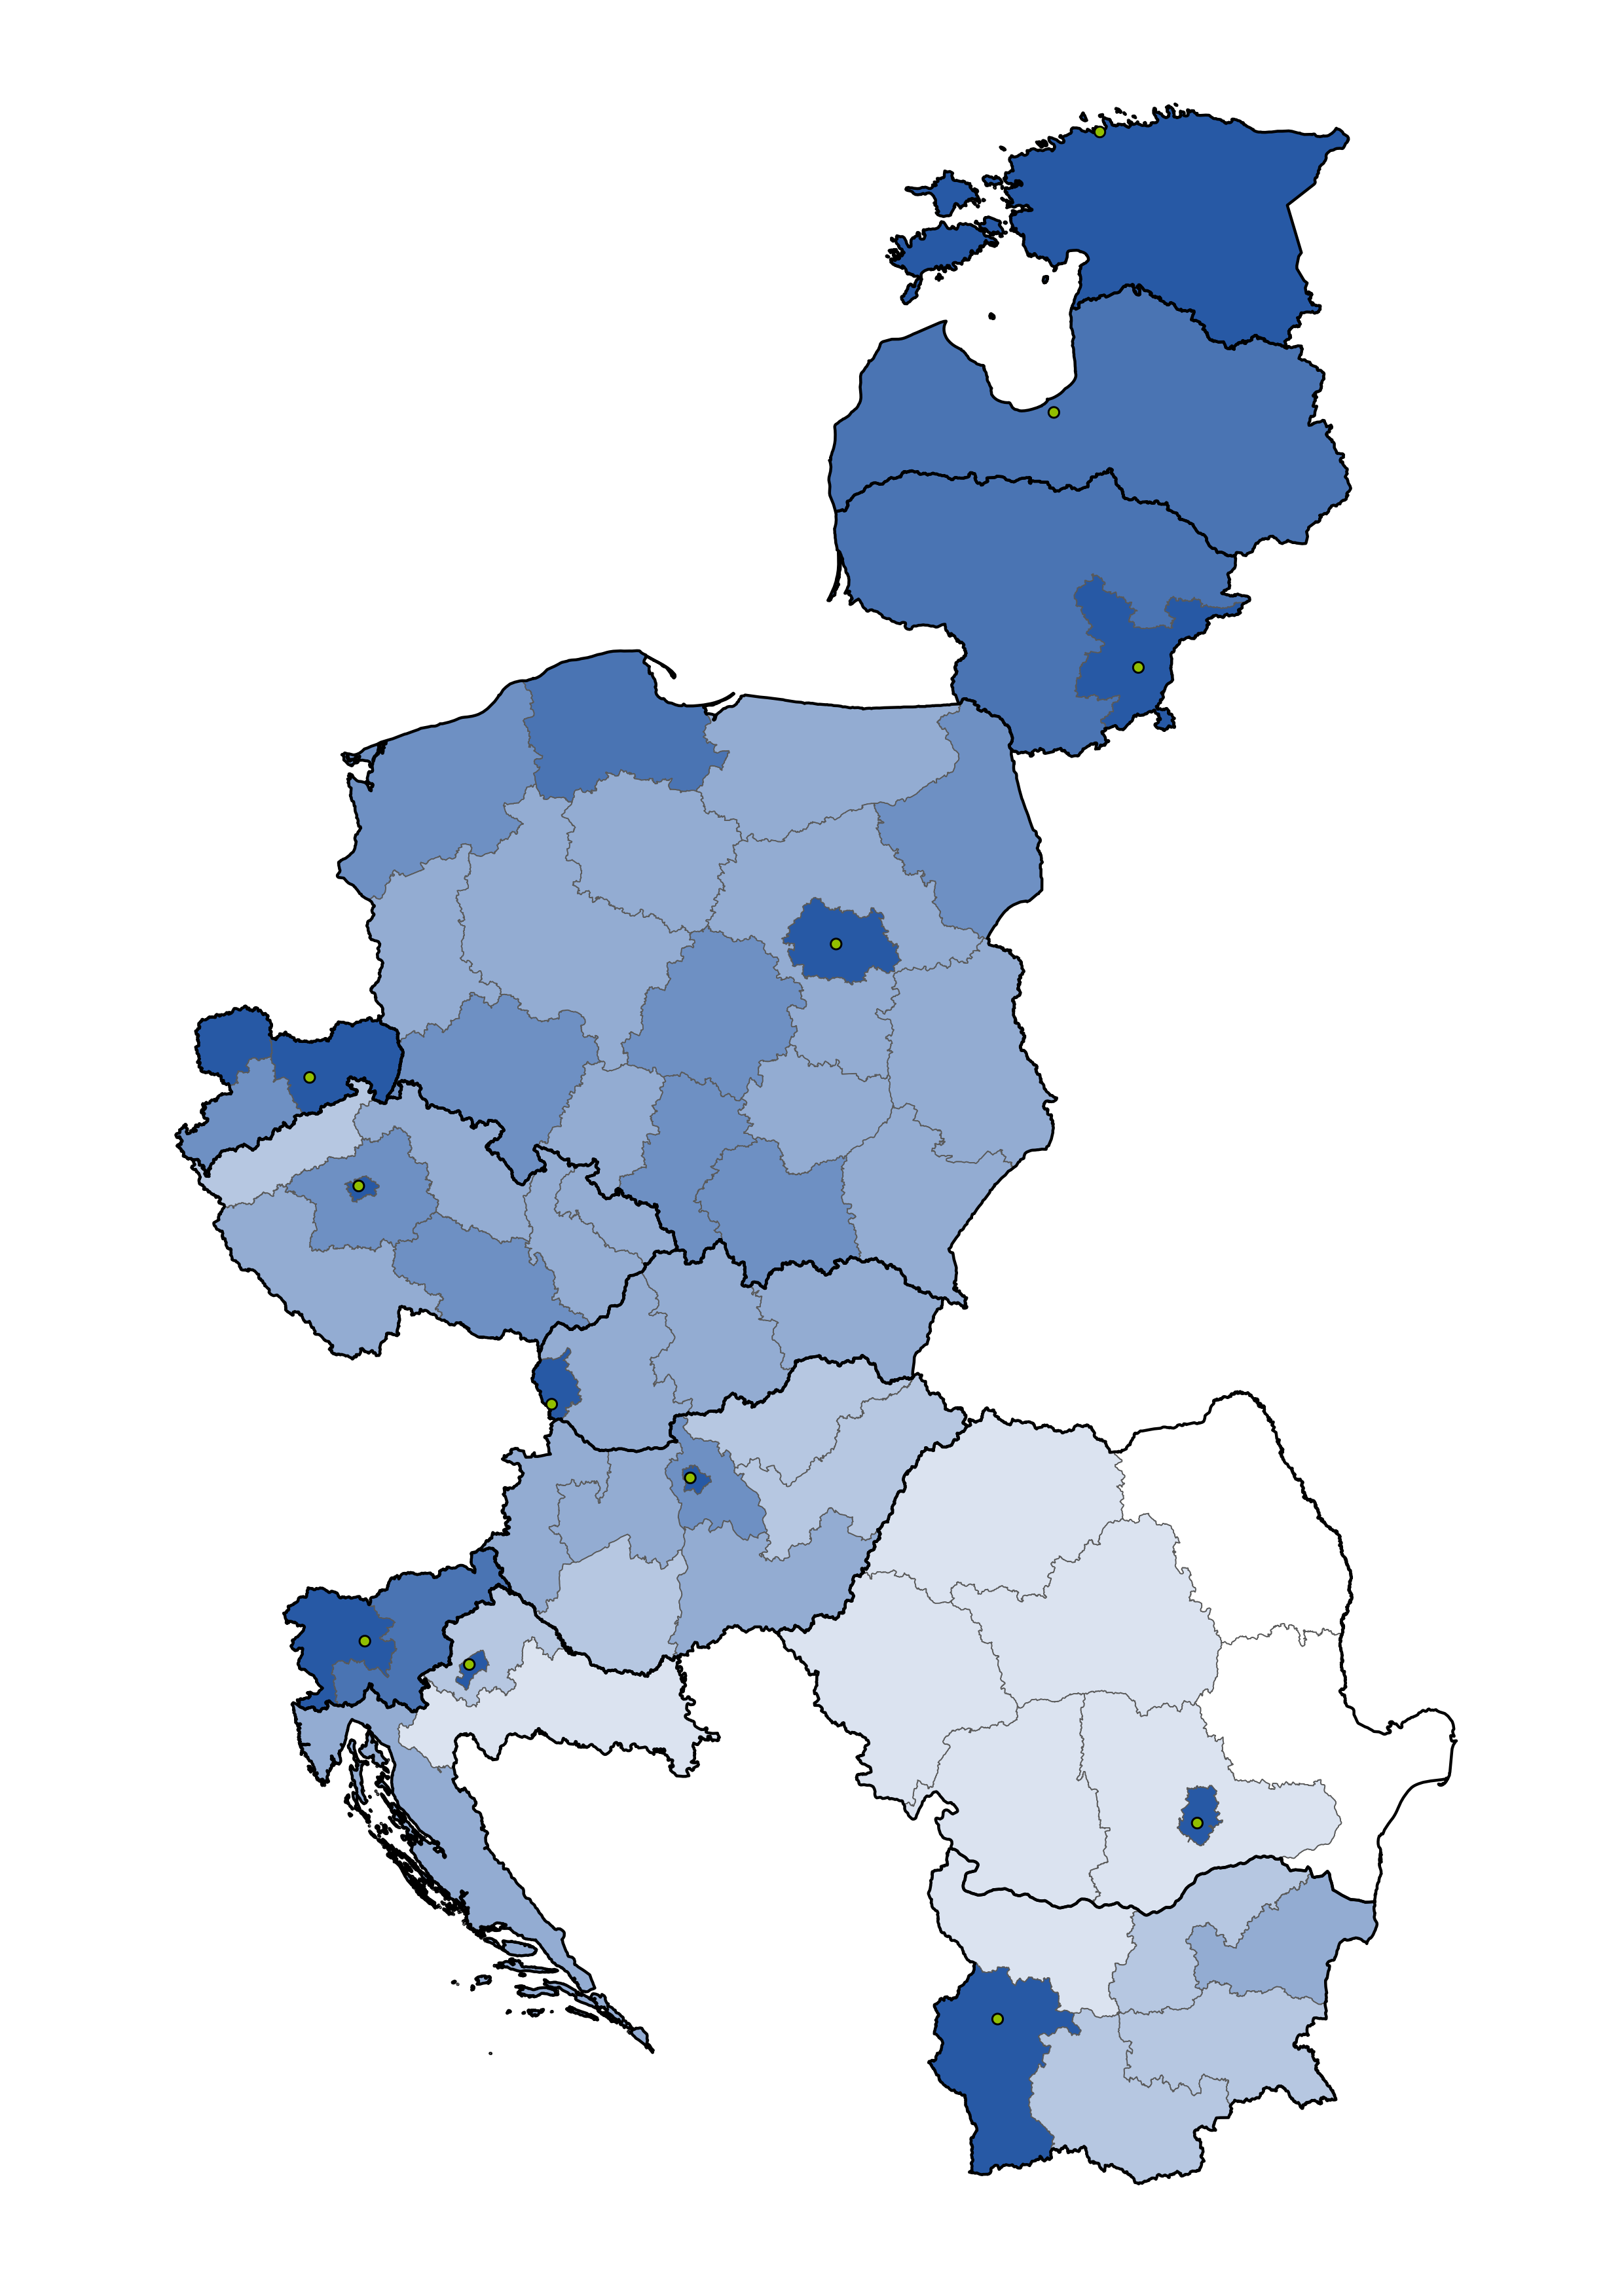
\includegraphics{Titelhindergrund}, angle=0, scale=1, opacity=.1}
		\BgThispage
		\restoregeometry
		\centering
		\vspace{2.5cm}
		{\color{imreg}\noindent\rule[1ex]{\textwidth}{11pt}\par}
		{\huge\bfseries Atlas zur M+E-Wirtschaft in Osteuropa\par}
		\vspace{1cm}
		{\color{imreg}\noindent\rule[1ex]{\textwidth}{11pt}\par}
		\vspace{2cm}
		{
\includegraphics[width=.5\textwidth]{imreg}\par}
		\vspace{2cm}
		{\scshape\Large\bfseries Langfassung\par}
		\vspace{1cm}
		{\scshape\Large\bfseries Aktualisierte Neuauflage\par}
		\vfill
		{\Large\itshape\bfseries Simon Gräfe\par}
		\vfill
		% Bottom of the page
		{\large\bfseries \monthyeardate\today \par}
		\vfill
	\end{titlepage}
	\restoregeometry
	
	\emptypage 
	\tableofcontents
	\newpage\listoftables
	\newpage\listoffigures
	\newpage\listofmaps
	
	\emptypage
	\include{Kapitel/Wertschöpfung}
	\emptypage
	%!TEX root = ../Osteuropaatlas.tex

\section{Wirtschaftliche Strukturdaten}


\setcounter{figure}{1}
\begin{figure}[!h]
	\addcontentsline{toc}{subsection}{IMD Wirtschaftsleistungsranking}
	\caption{IMD Wirtschaftsleistungsranking}
	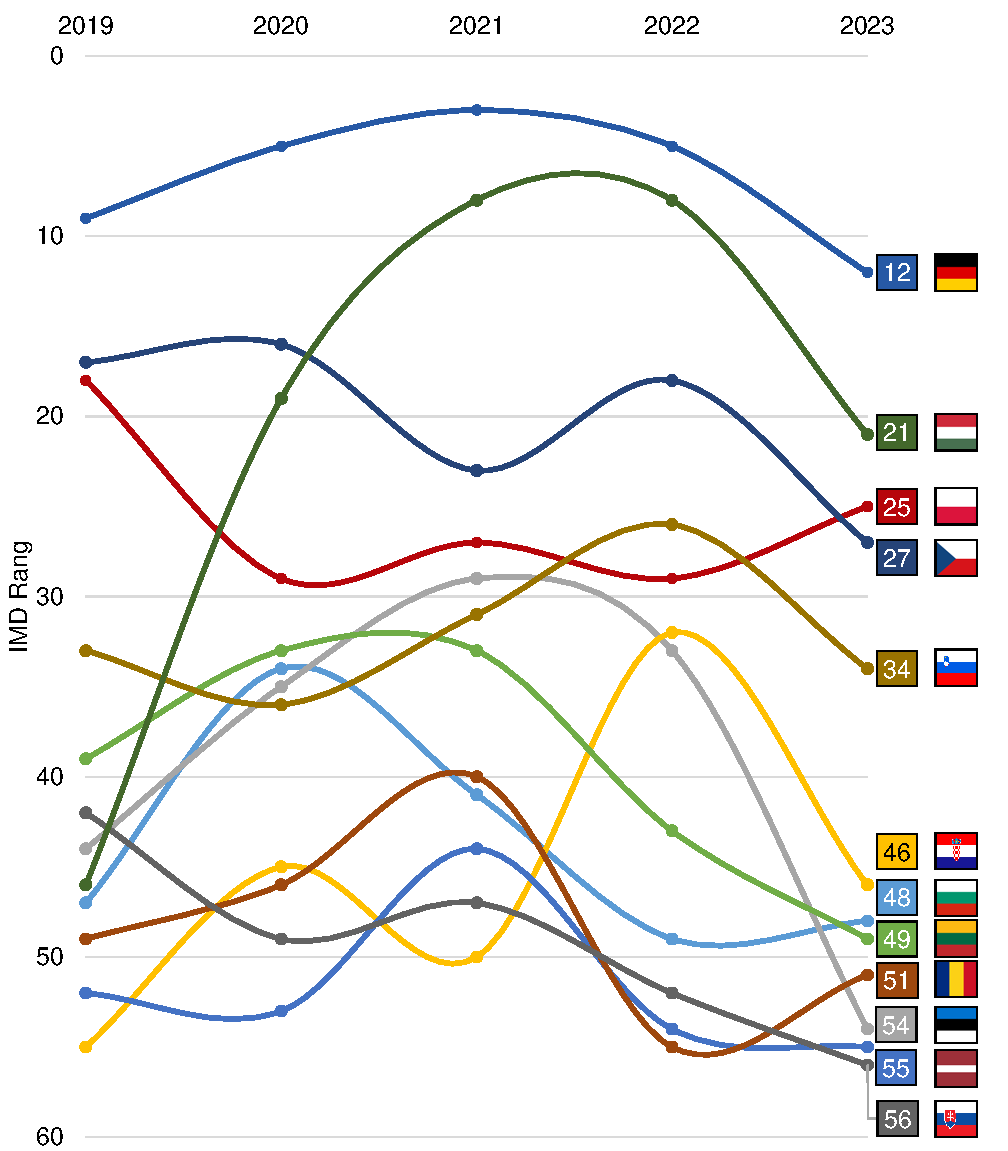
\includegraphics[width = \textwidth, height = 19.5cm]{IMD_Ranking}
	\begin{spacing}{1} \scriptsize
		\vspace{2mm}
		Anm.: IMD Economic Performance Ranking; Stand 2023\\
		Quelle: IMD World Competitiveness Center (2024); Dar. imreg (2024) \end{spacing}
\end{figure}


\begin{figure}[p]
	\addcontentsline{toc}{subsection}{Arbeitsstunden}
	{\centering \maps{Arbeitsstunden}}
	\label{map:stundengeleistet}
	\karte{Arbeitsstunden_geleistet}{2020}{Veränderung 2015 bis 2020}
	\begin{spacing}{1} \scriptsize
		Anm.: Jährliche Summe geleisteter Arbeitsstunden unabhängig von Bezahlung; Stand 2020\\
		Quelle: Eurostat (2024); Ber. \& Dar. imreg (2024) \end{spacing}
\end{figure}


\begin{figure}[p]
	\addcontentsline{toc}{subsection}{Arbeitsstunden je Erwerbstätigen}
	{\centering \maps{Arbeitsstunden je Erwerbstätigen}}
	\label{map:stundengeleistetprokopf}
	\karte{Arbeitsstunden_proErwerbstaetigen}{2020}{Veränderung 2015 bis 2020}
	\begin{spacing}{1} \scriptsize
		Anm.: Jährliche Summe geleisteter Arbeitsstunden unabhängig von Bezahlung; Stand 2020\\
		Quelle: Eurostat (2024); Ber. \& Dar. imreg (2024) \end{spacing}
\end{figure}


\begin{figure}[p]
	\addcontentsline{toc}{subsection}{Arbeitnehmerentgelt}
	{\centering \maps{Arbeitnehmerentgelt}}
	\label{map:entgelt}
	\karte{Arbeitnehmerentgelt}{2020}{Veränderung 2015 bis 2020}
	\begin{spacing}{1} \scriptsize
		Anm.: Jährliche Entgeltsumme; Stand 2020\\
		Quelle: Eurostat (2024); Ber. \& Dar. imreg (2024) \end{spacing}
\end{figure}


\begin{figure}[p]
	\addcontentsline{toc}{subsection}{Arbeitnehmerentgelt je Arbeitnehmer}
	{\centering \maps{Arbeitnehmerentgelt je Arbeitnehmer}}
	\label{map:entgeltprokopf}
	\karte{Entgelt_proKopf}{2020}{Veränderung 2015 bis 2020}
	\begin{spacing}{1} \scriptsize
		Anm.: Jährliche Entgeltsumme; Stand 2020\\
		Quelle: Eurostat (2024); Ber. \& Dar. imreg (2024) 
	\end{spacing}
\end{figure}


\begin{figure}[p]
	\addcontentsline{toc}{subsection}{Arbeitnehmerentgelt je Arbeitsstunde}
	{\centering \maps{Arbeitnehmerentgelt je Arbeitsstunde}}
	\label{map:entgeltprostunde}
	\karte{Entgelt_proH}{2020}{Veränderung 2015 bis 2020}
	\begin{spacing}{1} \scriptsize
		Anm.: Jährliche Entgeltsumme; Stand 2020\\
		Quelle: Eurostat (2024); Ber. \& Dar. imreg (2024) 
	\end{spacing}
\end{figure}


\begin{figure}[p]
	\addcontentsline{toc}{subsection}{Arbeitproduktivität je Erwerbestätigen (nominal)}
	{\centering \maps{Arbeitproduktivität je Erwerbestätigen (nominal)}}
	\label{map:prodprokopfnom}
	\karte{Arbeitsproduktivitaet_proErwerbstaetigen_nom}{2020}{Veränderung 2015 bis 2020}
	\begin{spacing}{1} \scriptsize
		Anm.: Jährlicher nominaler Produktionswert je Erwerbstätigen; Stand 2020\\
		Quelle: Eurostat (2024); Ber. \& Dar. imreg (2024) 
	\end{spacing}
\end{figure}


\begin{figure}[p]
	\addcontentsline{toc}{subsection}{Arbeitproduktivität je Arbeitsstunde (nominal)}
	{\centering \maps{Arbeitproduktivität je Arbeitsstunde (nominal)}}
	\label{map:prodprostundenom}
	\karte{Arbeitsproduktivitaet_proH_nom}{2020}{Veränderung 2015 bis 2020}
	\begin{spacing}{1} \scriptsize
		Anm.: Jährlicher nominaler Produktionswert je Arbeitsstunde; Stand 2020\\
		Quelle: Eurostat (2024); Ber. \& Dar. imreg (2024) 
	\end{spacing}
\end{figure}


\begin{figure}[p]
	\addcontentsline{toc}{subsection}{Entwicklung Arbeitsproduktivität (real)}
	{\centering \maps{Entwicklung Arbeitsproduktivität (real)}}
	\label{map:bipvol}
	\makebox[\linewidth][c]{
		\begin{subfigure}{0.61\textwidth}
			\centering
			\caption{Arbeitproduktivität je Erwerbestätigen (real)\\Veränderung 2015 bis 2020}
			\includegraphics[width=\textwidth, height=172mm, center]{Arbeitsproduktivitaet_proErwerbstaetigen_real_Delta} 
		\end{subfigure}
		\begin{subfigure}{0.61\textwidth}
			\centering
			\caption{Arbeitproduktivität je Arbeitsstunde (real)\\Veränderung 2015 bis 2020}
			\includegraphics[width=\textwidth, height=172mm, center]{Arbeitsproduktivitaet_proH_real_Delta}
		\end{subfigure}
	}
	\begin{spacing}{1} \scriptsize
		Anm.: Jährlicher nominaler Produktionswert je Erwerbestätigen/Arbeitsstunde Stand 2020\\
		Quelle: Eurostat (2024); Ber. \& Dar. imreg (2024) \end{spacing}
\end{figure}


\begin{figure}[p]
	\addcontentsline{toc}{subsection}{Anlageninvestitionen}
	{\centering \maps{Anlageninvestitionen}}
	\label{map:invest}
	\karte{Anlageninvestition}{2020}{Veränderung 2015 bis 2020}
	\begin{spacing}{1} \scriptsize
		Anm.: Anlageninvestitionen; Stand 2020\\
		Quelle: Eurostat (2024); Ber. \& Dar. imreg (2024) 
	\end{spacing}
\end{figure}


\begin{figure}[p]
	\addcontentsline{toc}{subsection}{Anzahl Unternehmen im Verarbeitenden Gewerbe}
	{\centering \maps{Anzahl Unternehmen im Verarbeitenden Gewerbe}}
	\label{map:unternehmenvg}
	\karte{StrukturVG_UntZahl}{2020}{Veränderung 2015 bis 2020}
	\begin{spacing}{1} \scriptsize
		Anm.: Stand 2020\\
		Quelle: Eurostat (2024); Ber. \& Dar. imreg (2024) 
	\end{spacing}
\end{figure}


\begin{figure}[p]
	\addcontentsline{toc}{subsection}{Anzahl Beschäftigter im Verarbeitenden Gewerbe}
	{\centering \maps{Anzahl Beschäftigter im Verarbeitenden Gewerbe}}
	\label{map:beschvg}
	\karte{StrukturVG_BeschZahl}{2020}{Veränderung 2015 bis 2020}
	\begin{spacing}{1} \scriptsize
		Anm.: Stand 2020\\
		Quelle: Eurostat (2024); Ber. \& Dar. imreg (2024) 
	\end{spacing}
\end{figure}


\begin{figure}[p]
	\addcontentsline{toc}{subsection}{Anteil Beschäftigter im Verarbeitenden Gewerbe an allen Beschäftigten}
	{\centering \maps{Anteil Beschäftigter im Verarbeitenden Gewerbe an allen Beschäftigten}}
	\label{map:beschanteilvg}
	\karte{Beschaeftigungsanteil_VG}{2022}{Veränderung 2015 bis 2022}
	\begin{spacing}{1} \scriptsize
		Anm.: Stand 2022\\
		Quelle: Eurostat (2024); Ber. \& Dar. imreg (2024) 
	\end{spacing}
\end{figure}


\begin{figure}[p]
	\addcontentsline{toc}{subsection}{Arbeitsstunden im Verarbeitenden Gewerbe}
	{\centering \maps{Arbeitsstunden im Verarbeitenden Gewerbe}}
	\label{map:stundengeleistetvg}
	\karte{Arbeitsstunden_geleistetVG}{2020}{Veränderung 2015 bis 2020}
	\begin{spacing}{1} \scriptsize
		Anm.: Jährliche Summe geleisteter Arbeitsstunden unabhängig von Bezahlung; Stand 2020\\
		Quelle: Eurostat (2024); Ber. \& Dar. imreg (2024) \end{spacing}
\end{figure}


\begin{figure}[p]
	\addcontentsline{toc}{subsection}{Arbeitnehmerentgelt im Verarbeitenden Gewerbe}
	{\centering \maps{Arbeitnehmerentgelt im Verarbeitenden Gewerbe}}
	\label{map:entgeltvg}
	\karte{Arbeitnehmerentgelt_VG}{2020}{Veränderung 2015 bis 2020}
	\begin{spacing}{1} \scriptsize
		Anm.: Jährliche Entgeltsumme; Stand 2020\\
		Quelle: Eurostat (2024); Ber. \& Dar. imreg (2024) \end{spacing}
\end{figure}

\begin{figure}[p]
	\addcontentsline{toc}{subsection}{Lohn \& Gehalt im Verarbeitenden Gewerbe}
	{\centering \maps{Lohn \& Gehalt im Verarbeitenden Gewerbe}}
	\label{map:entgeltvg2}
	\karte{StrukturVG_Lohn}{2020}{Veränderung 2015 bis 2020}
	\begin{spacing}{1} \scriptsize
		Anm.: Jährliche Lohn- \& Gehaltssumme; Stand 2020\\
		Quelle: Eurostat (2024); Ber. \& Dar. imreg (2024) \end{spacing}
\end{figure}


\begin{figure}[p]
	\addcontentsline{toc}{subsection}{Arbeitnehmerentgelt je Arbeitsstunde im Verarbeitenden Gewerbe}
	{\centering \maps{Arbeitnehmerentgelt je Arbeitsstunde im Verarbeitenden Gewerbe}}
	\label{map:entgeltprostundevg}
	\karte{Entgelt_proHVG}{2020}{Veränderung 2015 bis 2020}
	\begin{spacing}{1} \scriptsize
		Anm.: Jährliche Entgeltsumme; Stand 2020\\
		Quelle: Eurostat (2024); Ber. \& Dar. imreg (2024) 
	\end{spacing}
\end{figure}


\begin{figure}[p]
	\addcontentsline{toc}{subsection}{Anlageninvestitionen im Verarbeitenden Gewerbe}
	{\centering \maps{Anlageninvestitionen im Verarbeitenden Gewerbe}}
	\label{map:investvg}
	\karte{AnlageninvestitionVG}{2020}{Veränderung 2015 bis 2020}
	\begin{spacing}{1} \scriptsize
		Anm.: Anlageninvestitionen; Stand 2020\\
		Quelle: Eurostat (2024); Ber. \& Dar. imreg (2024) 
	\end{spacing}
\end{figure}


\begin{figure}[p]
	\addcontentsline{toc}{subsection}{Investitionsintensität im Verarbeitenden Gewerbe}
	{\centering \maps{Investitionsintensität im Verarbeitenden Gewerbe}}
	\label{map:investintenvg}
	\karte{InvestitionsintensitaetVG}{2020}{Veränderung 2015 bis 2020}
	\begin{spacing}{1} \scriptsize
		Anm.: Anlageninvestitionen je Beschäftigten; Stand 2020\\
		Quelle: Eurostat (2024); Ber. \& Dar. imreg (2024) 
	\end{spacing}
\end{figure}


	\emptypage
	%!TEX root = ../Osteuropaatlas.tex

\section{Arbeitsmarkt}

\begin{figure}[p]
	\addcontentsline{toc}{subsection}{Erwerbstätige}
	{\centering \maps{Erwerbstätige}}
	\label{map:erwerb}
	\karte{Erwerbstaetige}{2022}{Veränderung 2015 bis 2022}
	\begin{spacing}{1} \scriptsize
		Anm.: Personen im Alter von 15 bis 64 Jahre; Stand 2022\\
		Quelle: Eurostat (2024); Ber. \& Dar. imreg (2024) \end{spacing}
\end{figure}


\begin{figure}[p]
	\addcontentsline{toc}{subsection}{Erwerbstätigenquote}
	{\centering \maps{Erwerbstätigenquote}}
	\label{map:erwerbquote}
	\karte{Erwerbstaetigenquote}{2022}{Veränderung 2015 bis 2022}
	\begin{spacing}{1} \scriptsize
		Anm.: Anteil an Gesamtbevölkerung; Personen im Alter von 15 bis 64 Jahre; Stand 2022\\
		Quelle: Eurostat (2024); Ber. \& Dar. imreg (2024) \end{spacing}
\end{figure}


\begin{figure}[p]
	\addcontentsline{toc}{subsection}{Erwerbstätigenprognose}
	{\centering \maps{Erwerbstätigenprognose}}
	\label{map:erwerbprognose}
	\karte{Erwerbsbevoelkerungsprognose}{2050}{Veränderung 2024 bis 2050}
	\begin{spacing}{1} \scriptsize
		Anm.: Basisvorausberechnung; Personen im Alter von 15 bis 64 Jahre; Stand 2020\\
		Quelle: Eurostat (2024); Ber. \& Dar. imreg (2024) \end{spacing}
\end{figure}


\begin{figure}[p]
	\addcontentsline{toc}{subsection}{Teilzeitquote}
	{\centering \maps{Teilzeitquote}}
	\label{map:teilzeit}
	\karte{Teilzeitquote}{2022}{Veränderung 2015 bis 2022}
	\begin{spacing}{1} \scriptsize
		Anm.: Anteil an allen Erwerbstätigen; Personen im Alter von 15 bis 64 Jahre; Stand 2022\\
		Quelle: Eurostat (2024); Ber. \& Dar. imreg (2024) \end{spacing}
\end{figure}


\begin{figure}[p]
	\addcontentsline{toc}{subsection}{Erwerbstätigenquote Frauen}
	{\centering \maps{Erwerbstätigenquote Frauen}}
	\label{map:erwerbfrauen}
	\karte{Erwerbstaetigenquote_Frauen}{2022}{Veränderung 2015 bis 2022}
	\begin{spacing}{1} \scriptsize
		Anm.: Anteil an allen Frauen; Personen im Alter von 15 bis 64 Jahre; Stand 2022\\
		Quelle: Eurostat (2024); Ber. \& Dar. imreg (2024) \end{spacing}
\end{figure}


\begin{figure}[p]
	\addcontentsline{toc}{subsection}{Erwerbstätigenquote Männer}
	{\centering \maps{Erwerbstätigenquote Männer}}
	\label{map:erwerbmaenner}
	\karte{Erwerbstaetigenquote_Maenner}{2022}{Veränderung 2015 bis 2022}
	\begin{spacing}{1} \scriptsize
		Anm.: Anteil an allen Männern; Personen im Alter von 15 bis 64 Jahre; Stand 2022\\
		Quelle: Eurostat (2024); Ber. \& Dar. imreg (2024) \end{spacing}
\end{figure}


\begin{figure}[p]
	\addcontentsline{toc}{subsection}{Erwerbstätigenquote Niedrigqualifizierter}
	{\centering \maps{Erwerbstätigenquote Niedrigqualifizierter}}
	\label{map:erwerbniedrig}
	\karte{Erwerbstaetigenquote_Bildung02}{2022}{Veränderung 2015 bis 2022}
	\begin{spacing}{1} \scriptsize
		Anm.: Anteil an allen Niedrigqualifizierten; ISCED Stufen 0 bis 2; Personen im Alter von 15 bis 64 Jahre; Stand 2022\\
		Quelle: Eurostat (2024); Ber. \& Dar. imreg (2024) \end{spacing}
\end{figure}


\begin{figure}[p]
	\addcontentsline{toc}{subsection}{Erwerbstätigenquote Mittelqualifizierter}
	{\centering \maps{Erwerbstätigenquote Mittelqualifizierter}}
	\label{map:erwerbmittel}
	\karte{Erwerbstaetigenquote_Bildung34}{2022}{Veränderung 2015 bis 2022}
	\begin{spacing}{1} \scriptsize
		Anm.: Anteil an allen Mittelqualifizierten; ISCED Stufen 3 bis 4; Personen im Alter von 15 bis 64 Jahre; Stand 2022\\
		Quelle: Eurostat (2024); Ber. \& Dar. imreg (2024) \end{spacing}
\end{figure}

\begin{figure}[p]
	\addcontentsline{toc}{subsection}{Erwerbstätigenquote Hochqualifizierter}
	{\centering \maps{Erwerbstätigenquote Hochqualifizierter}}
	\label{map:erwerbhoch}
	\karte{Erwerbstaetigenquote_Bildung58}{2022}{Veränderung 2015 bis 2022}
	\begin{spacing}{1} \scriptsize
		Anm.: Anteil an allen Hochqualifizierten; ISCED Stufen 5 bis 8; Personen im Alter von 15 bis 64 Jahre; Stand 2022\\
		Quelle: Eurostat (2024); Ber. \& Dar. imreg (2024) \end{spacing}
\end{figure}


\begin{figure}[p]
	\addcontentsline{toc}{subsection}{Erwerbstätigenquote im Inland Geborener}
	{\centering \maps{Erwerbstätigenquote im Inland Geborener}}
	\label{map:erwerbinland}
	\karte{Erwerbstaetigenquote_Inlaender}{2022}{Veränderung 2015 bis 2022}
	\begin{spacing}{1} \scriptsize
		Anm.: Anteil an im Inland Geborenen; Geburtsland = Land der Erwerbstätigkeit; Personen im Alter von 15 bis 64 Jahre; Stand 2022\\
		Quelle: Eurostat (2024); Ber. \& Dar. imreg (2024) \end{spacing}
\end{figure}


\begin{figure}[p]
	\addcontentsline{toc}{subsection}{Erwerbstätigenquote im Ausland Geborener}
	{\centering \maps{Erwerbstätigenquote im Ausland Geborener}}
	\label{map:erwerbausland}
	\karte{Erwerbstaetigenquote_Auslaender}{2022}{Veränderung 2017 bis 2022}
	\begin{spacing}{1} \scriptsize
		Anm.: Anteil an im Ausland Geborenen; Geburtsland $\neq$ Land der Erwerbstätigkeit; Personen im Alter von 15 bis 64 Jahre; Stand 2022\\
		Quelle: Eurostat (2024); Ber. \& Dar. imreg (2024) \end{spacing}
\end{figure}


\begin{figure}[p]
	\addcontentsline{toc}{subsection}{Jugenderwerbstätigenquote}
	{\centering \maps{Jugenderwerbstätigenquote}}
	\label{map:erwerbjugend}
	\karte{Jugenderwerbstaetigenquote}{2022}{Veränderung 2015 bis 2022}
	\begin{spacing}{1} \scriptsize
		Anm.: Anteil an allen Jugendlichen; Personen im Alter von 15 bis 24 Jahre; Stand 2022\\
		Quelle: Eurostat (2024); Ber. \& Dar. imreg (2024) \end{spacing}
\end{figure}


\begin{figure}[p]
	\addcontentsline{toc}{subsection}{Erwerbspersonen}
	{\centering \maps{Erwerbspersonen}}
	\label{map:erwerbspers}
	\karte{Erwerbspersonen}{2022}{Veränderung 2015 bis 2022}
	\begin{spacing}{1} \scriptsize
		Anm.: Erwerbspersonen = Berufstätige \& Arbeitslose; Personen ab 15 Jahre; Stand 2022\\
		Quelle: Eurostat (2024); Ber. \& Dar. imreg (2024) \end{spacing}
\end{figure}


\begin{figure}[p]
	\addcontentsline{toc}{subsection}{Weibliche Erwerbspersonen}
	{\centering \maps{Weibliche Erwerbspersonen}}
	\label{map:erwerbspersfrauen}
	\karte{Erwerbspersonen_Frauen}{2022}{Veränderung 2015 bis 2022}
	\begin{spacing}{1} \scriptsize
		Anm.: Erwerbspersonen = Berufstätige \& Arbeitslose; Personen ab 15 Jahre; Stand 2022\\
		Quelle: Eurostat (2024); Ber. \& Dar. imreg (2024) \end{spacing}
\end{figure}


\begin{figure}[p]
	\addcontentsline{toc}{subsection}{Männliche Erwerbspersonen}
	{\centering \maps{Männliche Erwerbspersonen}}
	\label{map:erwerbspersmaenner}
	\karte{Erwerbspersonen_Maenner}{2022}{Veränderung 2015 bis 2022}
	\begin{spacing}{1} \scriptsize
		Anm.: Erwerbspersonen = Berufstätige \& Arbeitslose; Personen ab 15 Jahre; Stand 2022\\
		Quelle: Eurostat (2024); Ber. \& Dar. imreg (2024) \end{spacing}
\end{figure}


\begin{figure}[p]
	\addcontentsline{toc}{subsection}{Niedrigqualizifierte Erwerbspersonen}
	{\centering \maps{Niedrigqualizifierte Erwerbspersonen}}
	\label{map:erwerbspersniedrig}
	\karte{Erwerbspersonen_Bildung02}{2022}{Veränderung 2015 bis 2022}
	\begin{spacing}{1} \scriptsize
		Anm.: Erwerbspersonen = Berufstätige \& Arbeitslose; ISCED Stufen 0 bis 2; Personen ab 15 Jahre; Stand 2022\\
		Quelle: Eurostat (2024); Ber. \& Dar. imreg (2024) \end{spacing}
\end{figure}


\begin{figure}[p]
	\addcontentsline{toc}{subsection}{Mittelqualifizierte Erwerbspersonen}
	{\centering \maps{Mittelqualifizierte Erwerbspersonen}}
	\label{map:erwerbspersmittel}
	\karte{Erwerbspersonen_Bildung34}{2022}{Veränderung 2015 bis 2022}
	\begin{spacing}{1} \scriptsize
		Anm.: Erwerbspersonen = Berufstätige \& Arbeitslose; ISCED Stufen 3 bis 4; Personen ab 15 Jahre; Stand 2022\\
		Quelle: Eurostat (2024); Ber. \& Dar. imreg (2024) \end{spacing}
\end{figure}


\begin{figure}[p]
	\addcontentsline{toc}{subsection}{Hochqualifizierte Erwerbspersonen}
	{\centering \maps{Hochqualifizierte Erwerbspersonen}}
	\label{map:erwerbspershoch}
	\karte{Erwerbspersonen_Bildung58}{2022}{Veränderung 2015 bis 2022}
	\begin{spacing}{1} \scriptsize
		Anm.: Erwerbspersonen = Berufstätige \& Arbeitslose; ISCED Stufen 5 bis 8; Personen ab 15 Jahre; Stand 2022\\
		Quelle: Eurostat (2024); Ber. \& Dar. imreg (2024) \end{spacing}
\end{figure}


\begin{figure}[p]
	\addcontentsline{toc}{subsection}{Arbeitslosenquote}
	{\centering \maps{Arbeitslosenquote}}
	\label{map:arbeitslosenquote}
	\karte{Arbeitslosenquote}{2022}{Veränderung 2015 bis 2022}
	\begin{spacing}{1} \scriptsize
		Anm.: Personen im Alter von 15 bis 74 Jahren; Stand 2022\\
		Quelle: Eurostat (2024); Ber. \& Dar. imreg (2024) \end{spacing}
\end{figure}


\begin{figure}[p]
	\addcontentsline{toc}{subsection}{Arbeitslosenquote Frauen}
	{\centering \maps{Arbeitslosenquote Frauen}}
	\label{map:arbeitslosenquotefrauen}
	\karte{Arbeitslosenquote_Frauen}{2022}{Veränderung 2015 bis 2022}
	\begin{spacing}{1} \scriptsize
		Anm.: Personen im Alter von 15 bis 74 Jahren; Stand 2022\\
		Quelle: Eurostat (2024); Ber. \& Dar. imreg (2024) \end{spacing}
\end{figure}


\begin{figure}[p]
	\addcontentsline{toc}{subsection}{Arbeitslosenquote Männer}
	{\centering \maps{Arbeitslosenquote Männer}}
	\label{map:arbeitslosenquotemaenner}
	\karte{Arbeitslosenquote_Maenner}{2022}{Veränderung 2015 bis 2022}
	\begin{spacing}{1} \scriptsize
		Anm.: Personen im Alter von 15 bis 74 Jahren; Stand 2022\\
		Quelle: Eurostat (2024); Ber. \& Dar. imreg (2024) \end{spacing}
\end{figure}


\begin{figure}[p]
	\addcontentsline{toc}{subsection}{Arbeitslosenquote Niedrigqualifizierter}
	{\centering \maps{Arbeitslosenquote Niedrigqualifizierter}}
	\label{map:arbeitslosenquoteniedrig}
	\karte{Arbeitslosenquote_Bildung02}{2022}{Veränderung 2015 bis 2022}
	\begin{spacing}{1} \scriptsize
		Anm.: ISCED Stufen 0 bis 2; Personen im Alter von 15 bis 74 Jahren; Stand 2022\\
		Quelle: Eurostat (2024); Ber. \& Dar. imreg (2024) \end{spacing}
\end{figure}


\begin{figure}[p]
	\addcontentsline{toc}{subsection}{Arbeitslosenquote Mittelqualifizierter}
	{\centering \maps{Arbeitslosenquote Mittelqualifizierter}}
	\label{map:arbeitslosenquotemittel}
	\karte{Arbeitslosenquote_Bildung34}{2022}{Veränderung 2015 bis 2022}
	\begin{spacing}{1} \scriptsize
		Anm.: ISCED Stufen 3 bis 4; Personen im Alter von 15 bis 74 Jahren; Stand 2022\\
		Quelle: Eurostat (2024); Ber. \& Dar. imreg (2024) \end{spacing}
\end{figure}


\begin{figure}[p]
	\addcontentsline{toc}{subsection}{Arbeitslosenquote Hochqualifizierter}
	{\centering \maps{Arbeitslosenquote Hochqualifizierter}}
	\label{map:arbeitslosenquotehoch}
	\karte{Arbeitslosenquote_Bildung58}{2022}{Veränderung 2015 bis 2022}
	\begin{spacing}{1} \scriptsize
		Anm.: ISCED Stufen 5 bis 8; Personen im Alter von 15 bis 74 Jahren; Stand 2022\\
		Quelle: Eurostat (2024); Ber. \& Dar. imreg (2024) \end{spacing}
\end{figure}


\begin{figure}[p]
	\addcontentsline{toc}{subsection}{Ungenutzes Arbeitsmarktpotential}
	{\centering \maps{Ungenutzes Arbeitsmarktpotential}}
	\label{map:potential}
	\karte{Arbeitsmarktpotential}{2022}{Veränderung 2015 bis 2022}
	\begin{spacing}{1} \scriptsize
		Anm.: Anteil an der erweiterten Erwerbsbevölkerung; Personen im Alter von mind. 15 Jahren; Stand 2022\\
		Quelle: Eurostat (2024); Ber. \& Dar. imreg (2024) \end{spacing}
\end{figure}


\begin{figure}[p]
	\addcontentsline{toc}{subsection}{Ungenutzes Arbeitsmarktpotential Frauen}
	{\centering \maps{Ungenutzes Arbeitsmarktpotential Frauen}}
	\label{map:potentialfrauen}
	\karte{Arbeitsmarktpotential_Frauen}{2022}{Veränderung 2015 bis 2022}
	\begin{spacing}{1} \scriptsize
		Anm.: Anteil an der erweiterten weiblichen Erwerbsbevölkerung; Personen im Alter von mind. 15 Jahren; Stand 2022\\
		Quelle: Eurostat (2024); Ber. \& Dar. imreg (2024) \end{spacing}
\end{figure}


\begin{figure}[p]
	\addcontentsline{toc}{subsection}{Ungenutzes Arbeitsmarktpotential Männer}
	{\centering \maps{Ungenutzes Arbeitsmarktpotential Männer}}
	\label{map:potentialmaenner}
	\karte{Arbeitsmarktpotential_Maenner}{2022}{Veränderung 2015 bis 2022}
	\begin{spacing}{1} \scriptsize
		Anm.: Anteil an der erweiterten männlichen Erwerbsbevölkerung; Personen im Alter von mind. 15 Jahren; Stand 2022\\
		Quelle: Eurostat (2024); Ber. \& Dar. imreg (2024) \end{spacing}
\end{figure}


\begin{figure}[p]
	\addcontentsline{toc}{subsection}{Arbeitsmarktnachfrage IKT}
	{\centering \maps{Arbeitsmarktnachfrage IKT}}
	\label{map:ikt}
	\karte{Arbeitsmarktnachfrage_IKT}{2023}{Veränderung 2019-Q4 bis 2023-Q3}
	\begin{spacing}{1} \scriptsize
		Anm.: Anteil an Online-Stellenanzeigen; Stand 2023\\
		Quelle: Eurostat (2024); Ber. \& Dar. imreg (2024) \end{spacing}
\end{figure}


\begin{figure}[p]
	\addcontentsline{toc}{subsection}{Wochenarbeitszeit}
	{\centering \maps{Wochenarbeitszeit}}
	\label{map:zeit}
	\karte{Arbeitszeit}{2022}{Veränderung 2015 bis 2022}
	\begin{spacing}{1} \scriptsize
		Anm.: Vertragliche Wochenarbeitszeit; Personen im Alter von 15 bis 64 Jahre; Stand 2022\\
		Quelle: Eurostat (2024); Ber. \& Dar. imreg (2024) \end{spacing}
\end{figure}


\begin{figure}[p]
	\addcontentsline{toc}{subsection}{Langzeitbeschäftigung}
	{\centering \maps{Langzeitbeschäftigung}}
	\label{map:lang}
	\karte{Langzeitbeschaeftigung}{2022}{Veränderung 2015 bis 2022}
	\begin{spacing}{1} \scriptsize
		Anm.: Anteil Beschäftigungsverhältnisse mit mind. fünf Jahren Vertragsbestehen/ -dauer; Personen im Alter von 15 bis 64 Jahre; Stand 2022\\
		Quelle: Eurostat (2024); Ber. \& Dar. imreg (2024) \end{spacing}
\end{figure}


\begin{figure}[p]
	\addcontentsline{toc}{subsection}{Geschlechtsspezifischer Beschäftigungsunterschied}
	{\centering \maps{Geschlechtsspezifischer Beschäftigungsunterschied}}
	\label{map:geschlecht}
	\karte{Geschlechterbeschaeftigung}{2022}{Veränderung 2015 bis 2022}
	\begin{spacing}{1} \scriptsize
		Anm.: Unterschied Erwerbstätigenquote Männer zu Frauen im Alter von 20 bis 64 Jahre; Stand 2022\\
		Quelle: Eurostat (2024); Ber. \& Dar. imreg (2024) \end{spacing}
\end{figure}

	\emptypage
	%!TEX root = ../Osteuropaatlas.tex

\section{Metall \& Elektroindustrie}

\begin{table}[!h]
	\addcontentsline{toc}{subsection}{Strukturdaten der M+E-Wirtschaft in Osteuropa}
	\caption{Strukturdaten der M+E-Wirtschaft in Osteuropa}
	\begin{tblr}{
			width = \linewidth,
			rowsep = 4pt,
			colspec = {|X[l,m]|X[r,m]|X[r,m]|X[r,m]|X[r,m]|X[r,m]|},
			row{even} = {bg=imreg!20},
			row{1,2} = {c,bg=imreg,fg=white,font=\bfseries\large, rowsep=4pt},
			row{X} = {font=\bfseries}
			}
		\hline
		\SetCell[r=2]{m} Land & Betriebe (2022) & Beschäftigte (2022) & $\Sigma$ Entgelte (2021) & Umsatz (2022) & {Bruttowert-\\schöpfung (2021)}  \\
		\hline
		& Anzahl & Anzahl & Mio. EUR & Mio. EUR & Mio. EUR \\
		\hline
		Bulgarien & 9.934 & 197.856 & 1.870 & 23.310 & 3.680 \\
		\hline
		Estland & 3.742 & 46.008 & 701 & 7.237 & 1.491 \\
		\hline
		Kroatien & 10.717 & 97.422 & 1.154 & 8.693 & 2.321 \\
		\hline
		Lettland & 3.484 & 34.227 & 1.037 & 3.638 & 768 \\
		\hline
		Litauen & 7.824 & 72.735 & 486 & 7.307 & 2.029 \\
		\hline
		Polen & 120.002 & 1.264.882 & 16.349 & 216.166 & 42.498 \\
		\hline
		Rumänien & 24.972 & 484.698 & 6.620 & 59.839 & 11.960 \\
		\hline
		Slowakei & 50.861 & 302.823 & 4.488 & 71.005 & 11.908 \\
		\hline
		Slowenien & 10.341 & 128.176 & 2.731 & 25.148 & 5.807 \\
		\hline
		Tschechien & 101.034 & 810.191 & 13.054 & 155.711 & 28.127 \\
		\hline
		Ungarn & 30.979 & 441.020 & 6.559 & 89.351 & 15.152 \\
		\hline
		$\Sigma$ Osteuropa & 373.890 & 3.880.038 & 55.049 & 667.405 & 125.743 \\
		\hline
		Sachsen & 1.738 & 190.784 & 8.327 & 57.299 &  \\
		\hline
		Verhältnis Sachsen/ Osteuropa & 0,5\% & 4,9\% & 15,1\% & 8,6\% &  \\
		\hline
	\end{tblr}
	\begin{spacing}{1} \scriptsize
		\vspace{2mm}
		Anm.: WZ 24-30, 32+33; Betriebe ab einem Beschäftigten; Stand 2022\\
		Quelle: Eurostat (2024); Ber. \& Dar. imreg (2024) 
	\end{spacing}
\end{table}

\begin{figure}[p]
	\addcontentsline{toc}{subsection}{M+E-Beschäftigtenzahl}
	{\centering \maps{M+E-Beschäftigtenzahl}}
	\label{map:mebesch}
	\karte{ME_Besch}{2021}{Veränderung 2015 bis 2021}
	\begin{spacing}{1} \scriptsize
		Anm.: Stand 2021\\
		Quelle: Eurostat (2024); Ber. \& Dar. imreg (2024) \end{spacing}
\end{figure}


\begin{figure}[p]
	\addcontentsline{toc}{subsection}{M+E-Unternehmenszahl}
	{\centering \maps{M+E-Unternehmenszahl}}
	\label{map:meunt}
	\karte{ME_Unt}{2021}{Veränderung 2015 bis 2021}
	\begin{spacing}{1} \scriptsize
		Anm.: Stand 2021\\
		Quelle: Eurostat (2024); Ber. \& Dar. imreg (2024) \end{spacing}
\end{figure}


\begin{figure}[p]
	\addcontentsline{toc}{subsection}{M+E-Lohn- \& Gehaltssumme}
	{\centering \maps{M+E-Lohn- \& Gehaltssumme}}
	\label{map:melohn}
	\karte{ME_Entgelt}{2021}{Veränderung 2015 bis 2021}
	\begin{spacing}{1} \scriptsize
		Anm.: Stand 2021\\
		Quelle: Eurostat (2024); Ber. \& Dar. imreg (2024) \end{spacing}
\end{figure}


\begin{figure}[p]
	\addcontentsline{toc}{subsection}{M+E-Beschäftigte je Betrieb}
	{\centering \maps{M+E-Beschäftigte je Betrieb}}
	\label{map:mebschdichte}
	\karte{ME_BeschProBetrieb}{2021}{Veränderung 2015 bis 2021}
	\begin{spacing}{1} \scriptsize
		Anm.: Stand 2021\\
		Quelle: Eurostat (2024); Ber. \& Dar. imreg (2024) \end{spacing}
\end{figure}


\begin{figure}[p]
	\addcontentsline{toc}{subsection}{M+E-Beschäftigte je Tsd. Einwohner}
	{\centering \maps{M+E-Beschäftigte je Tsd. Einwohner}}
	\label{map:mebschdichteew}
	\karte{ME_BeschProEW}{2021}{Veränderung 2015 bis 2021}
	\begin{spacing}{1} \scriptsize
		Anm.: Stand 2021\\
		Quelle: Eurostat (2024); Ber. \& Dar. imreg (2024) \end{spacing}
\end{figure}


\begin{figure}[p]
	\addcontentsline{toc}{subsection}{M+E-Beschäftigte je Tsd. Einwohner}
	{\centering \maps{Anteil M+E-Beschäftigter an allen Industriebeschäftigten}}
	\label{map:mebeschanteil}
	\karte{ME_AnteilBeschVG}{2020}{Veränderung 2015 bis 2020}
	\begin{spacing}{1} \scriptsize
		Anm.: Anteil an allen Beschäftigten im Verarbeitenden Gewerbe; Stand 2020\\
		Quelle: Eurostat (2024); Ber. \& Dar. imreg (2024) \end{spacing}
\end{figure}
	\emptypage
	%!TEX root = ../Osteuropaatlas.tex

\section{Forschung \& Entwicklung}

\begin{figure}[p]
	\addcontentsline{toc}{subsection}{Ausgabenanteil in Forschung \& Entwicklung}
	{\centering \maps{Ausgabenanteil in Forschung \& Entwicklung}}
	\label{map:forschausgaben}
	\karte{FuEAusgaben}{2021}{Veränderung 2017 bis 2021}
	\begin{spacing}{1} \scriptsize
		Anm.: Anteil am BIP; Stand 2021\\
		Quelle: Eurostat (2024); Ber. \& Dar. imreg (2024) \end{spacing}
\end{figure}


\begin{figure}[p]
	\addcontentsline{toc}{subsection}{Forscheranteil}
	{\centering \maps{Forscheranteil}}
	\label{map:forscher}
	\karte{Forscher}{2021}{Veränderung 2015 bis 2021}
	\begin{spacing}{1} \scriptsize
		Anm.: Anteil an allen Erwerbstätigen in Vollzeitäquivalenten; Stand 2021\\
		Quelle: Eurostat (2024); Ber. \& Dar. imreg (2024) \end{spacing}
\end{figure}


\begin{figure}[p]
	\addcontentsline{toc}{subsection}{Anteil Forscher in Unternehmen}
	{\centering \maps{Anteil Forscher in Unternehmen}}
	\label{map:forscherunt}
	\karte{Forscher_Unternehmen}{2021}{Veränderung 2015 bis 2021}
	\begin{spacing}{1} \scriptsize
		Anm.: Anteil an allen Erwerbstätigen in Vollzeitäquivalenten; Stand 2021\\
		Quelle: Eurostat (2024); Ber. \& Dar. imreg (2024) \end{spacing}
\end{figure}


\begin{figure}[p]
	\addcontentsline{toc}{subsection}{Anteil Forscher an Hochschulen}
	{\centering \maps{Anteil Forscher an Hochschulen}}
	\label{map:forscherhoch}
	\karte{Forscher_Hochschule}{2021}{Veränderung 2015 bis 2021}
	\begin{spacing}{1} \scriptsize
		Anm.: Anteil an allen Erwerbstätigen in Vollzeitäquivalenten; Stand 2021\\
		Quelle: Eurostat (2024); Ber. \& Dar. imreg (2024) \end{spacing}
\end{figure}


\begin{figure}[p]
	\addcontentsline{toc}{subsection}{Anteil Forscher im Staatsdienst}
	{\centering \maps{Anteil Forscher im Staatsdienst}}
	\label{map:forscherstaat}
	\karte{Forscher_Staat}{2021}{Veränderung 2015 bis 2021}
	\begin{spacing}{1} \scriptsize
		Anm.: Anteil an allen Erwerbstätigen in Vollzeitäquivalenten; Stand 2021\\
		Quelle: Eurostat (2024); Ber. \& Dar. imreg (2024) \end{spacing}
\end{figure}
	\emptypage
	\include{Kapitel/Bevölkerungsstruktur}
	\emptypage
	\include{Kapitel/Sozioökonomische Daten}
	\emptypage
	%!TEX root = ../Osteuropaatlas.tex


\section{Einkommen}


\begin{figure}[p]
	{\centering \maps{Primäreinkommen}}
	\label{map:einkommenprim}
	\karte{Primaereinkommen}{2020}{Veränderung 2015 bis 2020}
	\begin{spacing}{1} \scriptsize
		Anm.: Nettoprimäreinkommen; $\text{Primaereinkommen = Einkommen $-$ Ausgaben durch Erwerbstätigkeit \& Vermögen}$; Stand 2020\\
		Quelle: Eurostat (2024); Ber. \& Dar. imreg (2024) \end{spacing}
\end{figure}


\begin{figure}[p]
	{\centering \maps{Verfügbares Einkommen}}
	\label{map:einkommenverf}
	\karte{VerfuegbaresEinkommen_Ausgaben}{2020}{Veränderung 2015 bis 2020}
	\begin{spacing}{1} \scriptsize
		Anm.: Verfügbares Einkommen = Einkommen nach Umverteilung; Berechnung nach dem Ausgabenkonzept; Stand 2020\\
		Quelle: Eurostat (2024); Ber. \& Dar. imreg (2024) \end{spacing}
\end{figure}


\begin{figure}[p]
	{\centering \maps{Betriebsüberschuss \& Selbstständigeneinkommen}}
	\label{map:einkommenbetrieb}
	\karte{Betriebsueberschuss}{2020}{Veränderung 2015 bis 2020}
	\begin{spacing}{1} \scriptsize
		Anm.: Nettbetriebsüberschuss \& -selbstständigeneinkommen; Stand 2020\\
		Quelle: Eurostat (2024); Ber. \& Dar. imreg (2024) \end{spacing}
\end{figure}


\begin{figure}[p]
	{\centering \maps{Arbeitnehmerentgelt}}
	\label{map:einkommenarbeit}
	\karte{Arbeitnehmerentgelt_Einkommen}{2020}{Veränderung 2015 bis 2020}
	\begin{spacing}{1} \scriptsize
		Anm.: Stand 2020\\
		Quelle: Eurostat (2024); Ber. \& Dar. imreg (2024) \end{spacing}
\end{figure}


\begin{figure}[p]
	{\centering \maps{Vermögenseinkommen}}
	\label{map:einkommenverm}
	\karte{Vermoegenseinkommen}{2020}{Veränderung 2015 bis 2020}
	\begin{spacing}{1} \scriptsize
		Anm.: Stand 2020\\
		Quelle: Eurostat (2024); Ber. \& Dar. imreg (2024) \end{spacing}
\end{figure}


\begin{figure}[p]
	{\centering \maps{Einkommen aus Sozialleistungen}}
	\label{map:einkommensozial}
	\karte{Sozialleistungen}{2020}{Veränderung 2015 bis 2020}
	\begin{spacing}{1} \scriptsize
		Anm.: Stand 2020\\
		Quelle: Eurostat (2024); Ber. \& Dar. imreg (2024) \end{spacing}
\end{figure}


\begin{figure}[p]
	{\centering \maps{Einkommen aus sonstigen Transfers}}
	\label{map:einkommensonst}
	\karte{SonstTransfers}{2020}{Veränderung 2015 bis 2020}
	\begin{spacing}{1} \scriptsize
		Anm.: Siehe Europäisches System Volkswirtschaftlicher Gesamtrechnungen (ESVG); Stand 2020\\
		Quelle: Eurostat (2024); Ber. \& Dar. imreg (2024) \end{spacing}
\end{figure}


\begin{figure}[p]
	{\centering \maps{Steueraufkommen durch Einkommen \& Vermögen}}
	\label{map:einkommensteuer}
	\karte{SonstTransfers}{2020}{Veränderung 2015 bis 2020}
	\begin{spacing}{1} \scriptsize
		Anm.: Stand 2020\\
		Quelle: Eurostat (2024); Ber. \& Dar. imreg (2024) \end{spacing}
\end{figure}


\begin{figure}[p]
	{\centering \maps{Geleistete Sozialbeiträge}}
	\label{map:einkommenbeiträge}
	\karte{Sozialbeitraege}{2020}{Veränderung 2015 bis 2020}
	\begin{spacing}{1} \scriptsize
		Anm.: Stand 2020\\
		Quelle: Eurostat (2024); Ber. \& Dar. imreg (2024) \end{spacing}
\end{figure}
	\emptypage
	%!TEX root = ../Osteuropaatlas.tex

\section{Hinweise \& Definitionen}


Generell wird von M+E-Wirtschaft bzw. einem M+E-Gewerbe gesprochen, wenn alle Betriebe ab einem Beschäftigten erfasst sind. Unter M+E-Industrie dagegen werden nur diejenigen Einheiten mit 20 und mehr Beschäftigten verstanden.

\begin{table}[!h]
	\caption{Metall- und Elektroindustrie in der Wirtschaftszweigklassifikation 2008}
	\begin{tblr}{
				colspec = {|X|X|X|X|X|},
				columns = {font = \small},
				row{1} = {font = \small\bfseries, bg = lightgray!20},
				vlines = {1pt},
				vline{6} = {12-19}{imregdunkelrot, 1pt},
				vline{3,6} = {21-22}{imregdunkelrot, 1pt},
				vline{3} = {16-19}{imregdunkelrot, 1pt},
				vline{5} = {12-14}{imregdunkelrot, 1pt},
				vline{4} = {15}{imregdunkelrot, 1pt},
			}
		\hline
		1. Ebene & 2. Ebene & 3. Ebene & 4. Ebene & 5. Ebene \\
		\hline
		\SetCell[c=5]{l, font=\small\bfseries} Land- \& Forstwirtschaft (A) &  &  &  &  \\
		\hline
		\SetCell[r=23]{m, font=\small\bfseries, bg=imreg!20} Produzierendes Gewerbe (B-F) & \SetCell[c=4]{l} Bergbau (B) &  &  &  \\
		\hline
		& \SetCell[r=19]{m, bg=imreg!20} Verarbeitendes Gewerbe  (C) & \SetCell[c=3]{l} Nahrung \& Genuss (10-12) &  &  \\
		\hline
		&  & \SetCell[c=3]{l} Bekleidung (13-15) &  &  \\
		\hline
		&  & \SetCell[c=3]{l} Holz \& Papier (16-18) &  &  \\
		\hline
		&  & \SetCell[c=3]{l} Kokerei \& Mineralöl (19) &  &  \\
		\hline
		&  & \SetCell[c=3]{l} Chemie \& Pharma (20+21) &  &  \\
		\hline
		&  & \SetCell[c=3]{l} Gummi, Glas \& Kunststoffe (22+23) &  &  \\
		\hline
		&  & \SetCell[r=6]{m, fg=white, bg=imreg} Metallindustrie (24+25) & \SetCell[r=5]{m, fg=white, bg=imreg} Metallerzeugung \& -bearbeitung (24) & \SetCell{l, fg=white, bg=imreg} Roheisen, Stahl und Ferrolegierungen (24.1) \\
		\hline
		&  &  &  & \SetCell{l, fg=white, bg=imreg} Stahlerzeugnisse (24.2) \\
		\SetHline{5}{imregdunkelrot,1pt}
		&  &  &  & \SetCell{l, fg=white, bg=imreg} Sonst. erste Bearbeitung v. Eisen \& Stahl (24.3) \\
		\hline
		&  &  &  & \SetCell{l, fg=white, bg=imreg} Erzeugung und Bearbeitung von Nicht-Eisen-Metallen (24.4) \\
		\hline
		&  &  &  & \SetCell{l, fg=white, bg=imreg} Gießereien (24.5) \\
		\SetHline{4}{imregdunkelrot,1pt}
		&  &  & \SetCell[c=2]{l, fg=white, bg=imreg} Herstellung v. Metallerzeugnissen (25) &  \\
		\SetHline{3}{imregdunkelrot,1pt}
		&  & \SetCell[c=3]{l, fg=white, bg=imreg} Elektroindustrie (26+27) &  &  \\
		\hline
		&  & \SetCell[c=3]{l, fg=white, bg=imreg} Maschinenbau (28) &  &  \\
		\hline
		&  & \SetCell[c=3]{l, fg=white, bg=imreg} Fahrzeugbau (29) &  &  \\
		\hline
		&  & \SetCell[c=3]{l, fg=white, bg=imreg} Sonst. Fahrzeugbau (30) &  &  \\
		\SetHline{3-5}{imregdunkelrot,1pt}
		&  & \SetCell[c=3]{l} Möbel (31) &  &  \\
		\SetHline{3-5}{imregdunkelrot,1pt}
		&  & \SetCell[c=3]{l, fg=white, bg=imreg}Sonst. Herstellung von Waren (32) &  &  \\
		\hline
		&  & \SetCell[c=3]{l, fg=white, bg=imreg} Reparaturen \& Installationen (33) &  &  \\
		\SetHline{3-5}{imregdunkelrot,1pt}
		& \SetCell[c=4]{l} Energieversorgung (D) &  &  &  \\
		\hline
		& \SetCell[c=4]{l} Wasserversorgung ( E) &  &  &  \\
		\hline
		& \SetCell[c=4]{l} Bau (F) &  &  &  \\
		\hline
		\SetCell[c=5]{l, font=\small\bfseries} Dienstleistungen (G-U) &  &  &  &  \\
		\hline
	\end{tblr}
	\begin{spacing}{1} \scriptsize
		\vspace{2mm}
		Anm.: dunkelblau = M+E-Industrie im weiteren Sinn; rot = M+E-Industrie im engeren Sinn\\
		Quelle: Statistisches Bundesamt (2024); Dar. imreg (2024) \end{spacing}
\end{table}





\begin{table}
	\addcontentsline{toc}{subsection}{Übersicht der ausgewerteten Regionen nach NUTS-Systematik}
	\caption{Übersicht der ausgewerteten Regionen nach NUTS-Systematik}
	\begin{tblr}{
			width=\linewidth, 
			colspec={|X[-1,c]|X[-1,c]|X[l]|X[-1,c]|X[-1,c]|X[l]|},
%			rowsep = 0pt,
			row{odd} = {bg=imreg!20},
			row{1,2} = {c,bg=imreg,fg=white,font=\bfseries\large, rowsep=4pt},
			cell{3,17,21}{1} = {bg=white},
			cell{20,26}{1} = {bg=imreg!20},
			cell{3}{4} = {bg=white},
			cell{20,30}{4} = {bg=imreg!20}
		}
		\hline
		Land & \SetCell[c=2]{m} NUTS 2 Ebene &  & Land & \SetCell[c=2]{m} NUTS 2 Ebene &  \\
		\hline
		& Code & Name &  & Code & Name \\
		\hline
		\SetCell[r=6]{m} Bulgarien & BG31 & Severozapaden & \SetCell[r=17]{m} Polen & PL21 & Małopolskie \\
		\hline
		& BG32 & Severen tsentralen &  & PL22 & Śląskie \\
		\hline
		& BG33 & Severoiztochen &  & PL41 & Wielkopolskie \\
		\hline
		& BG34 & Yugoiztochen &  & PL42 & Zachodniopomorskie \\
		\hline
		& BG41 & Yugozapaden &  & PL43 & Lubuskie \\
		\hline
		& BG42 & Yuzhen tsentralen &  & PL51 & Dolnośląskie \\
		\hline
		\SetCell[r=8]{m} Tschechien & CZ01 & Praha &  & PL52 & Opolskie \\
		\hline
		& CZ02 & Střední Čechy &  & PL61 & Kujawsko-pomorskie \\
		\hline
		& CZ03 & Jihozápad &  & PL62 & Warmińsko-mazurskie \\
		\hline
		& CZ04 & Severozápad &  & PL63 & Pomorskie \\
		\hline
		& CZ05 & Severovýchod &  & PL71 & Łódzkie \\
		\hline
		& CZ06 & Jihovýchod &  & PL72 & Świętokrzyskie \\
		\hline
		& CZ07 & Střední Morava &  & PL81 & Lubelskie \\
		\hline
		& CZ08 & Moravskoslezsko &  & PL82 & Podkarpackie \\
		\hline
		\SetCell[r=3]{m} Deutschland & DED2 & Dresden &  & PL84 & Podlaskie \\
		\hline
		& DED4 & Chemnitz &  & PL91 & Warszawski stołeczny \\
		\hline
		& DED5 & Leipzig &  & PL92 & Mazowiecki regionalny \\
		\hline
		Estland & EE00 & Eesti & \SetCell[r=8]{m} Rumänien & RO11 & Nord-Vest \\
		\hline
		\SetCell[r=2]{m} Kroatien & HR03 & Jadranska Hrvatska &  & RO12 & Centru \\
		\hline
		& HR04 & Kontinentalna Hrvatska &  & RO21 & Nord-Est \\
		\hline
		Lettland & LV00 & Latvija &  & RO22 & Sud-Est \\
		\hline
		\SetCell[r=2]{m} Litauen & LT01 & Sostinės regionas &  & RO31 & Sud-Muntenia \\
		\hline
		& LT02 & Vidurio ir vakarų Lietuvos regionas  &  & RO32 & Bucureşti-Ilfov \\
		\hline
		\SetCell[r=8]{m} Ungarn & HU11 & Budapest &  & RO41 & Sud-Vest Oltenia \\
		\hline
		& HU12 & Pest &  & RO42 & Vest \\
		\hline
		& HU21 & Közép-Dunántúl & \SetCell[r=2]{m} Slowenien & SI03 & Vzhodna Slovenija \\
		\hline
		& HU22 & Nyugat-Dunántúl &  & SI04 & Zahodna Slovenija \\
		\hline
		& HU23 & Dél-Dunántúl & \SetCell[r=4]{m} Slowakei & SK01 & Bratislavský kraj \\
		\hline
		& HU31 & Észak-Magyarország &  & SK02 & Západné Slovensko \\
		\hline
		& HU32 & Észak-Alföld &  & SK03 & Stredné Slovensko \\
		\hline
		& HU33 & Dél-Alföld &  & SK04 & Východné Slovensko \\
		\hline
	\end{tblr}
	\begin{spacing}{1} \scriptsize
		\vspace{2mm}
		Quelle: Eurostat (2024); Dar. imreg (2024) 
	\end{spacing}
\end{table}


\begin{figure}[p]
	\addcontentsline{toc}{subsection}{Übersicht der NUTS-2-Regionen}
	{\centering \maps{Übersicht der NUTS-2-Regionen}}
	\label{map:nuts_systematik}
	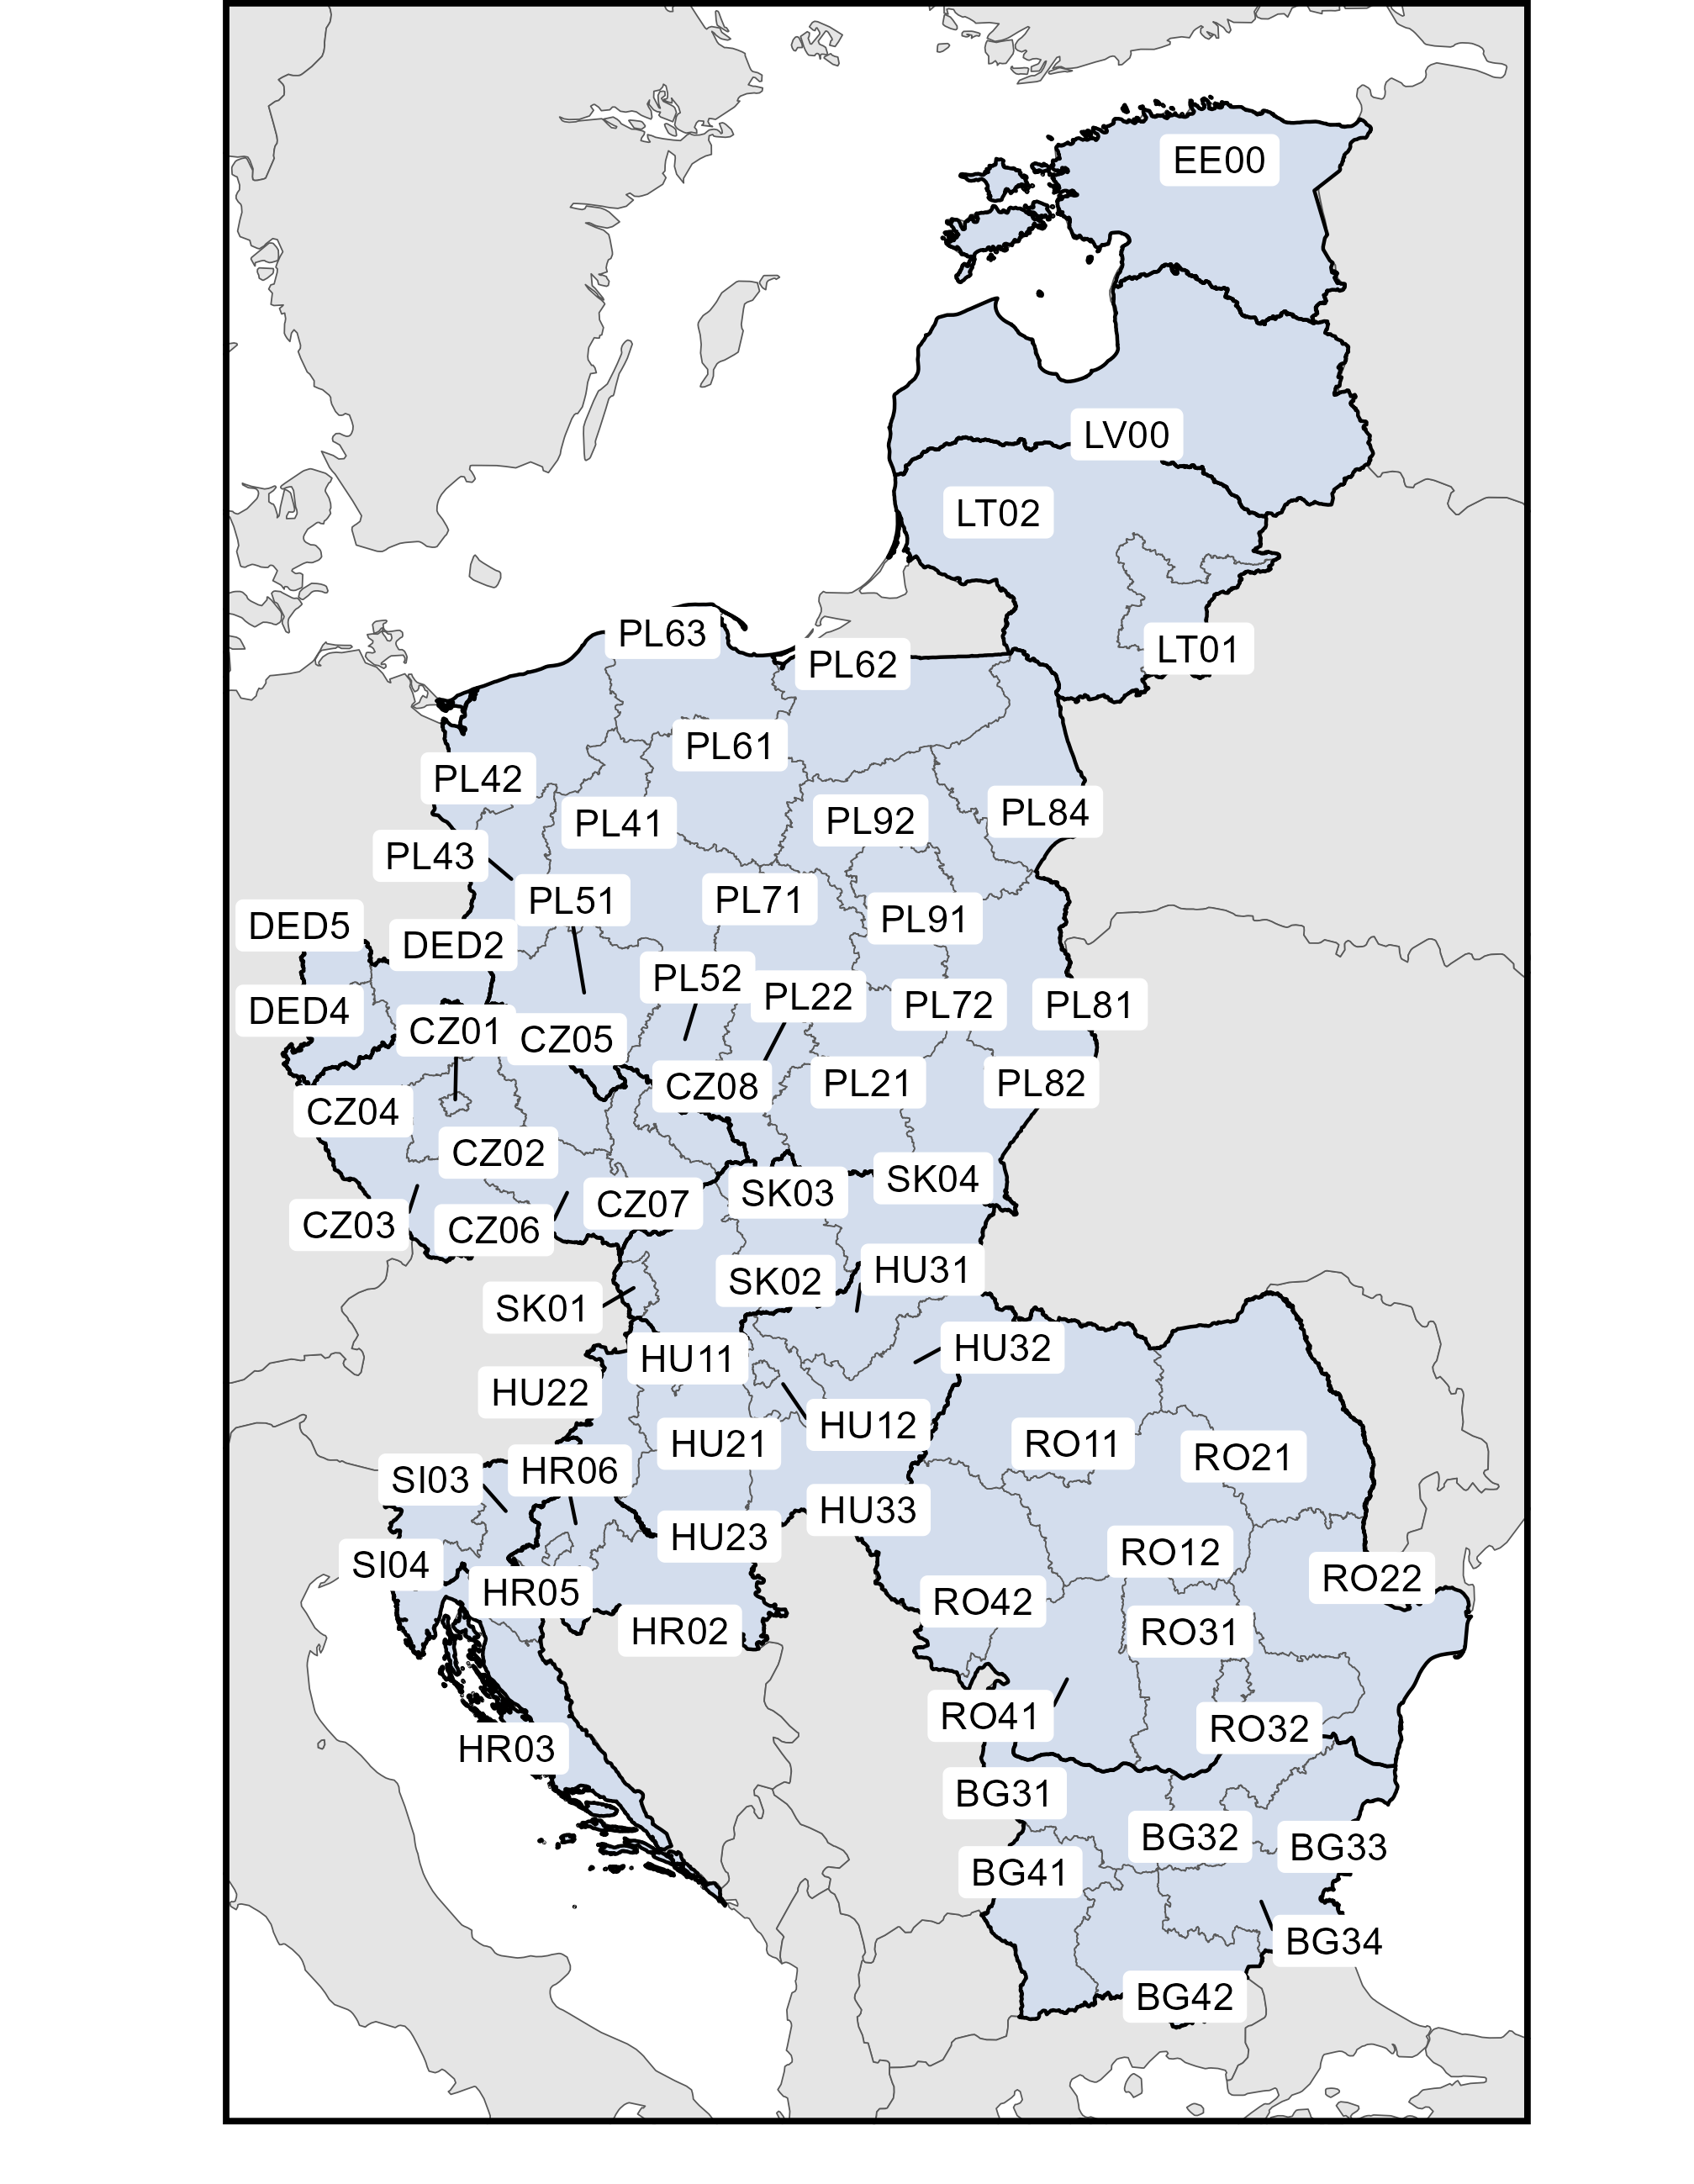
\includegraphics[width=\textwidth]{NUTS_Systematik}
	\begin{spacing}{1} \scriptsize
		Quelle: Eurostat (2024); Dar. imreg (2024) \end{spacing}
\end{figure}



	
\end{document}